\documentclass[a4paper, 12pt]{article}
\usepackage[utf8x]{inputenc}
\usepackage[english, russian]{babel}
\usepackage[left=25mm, top=25mm, right=25mm, bottom=25mm]{geometry}
\usepackage{cmap}
\usepackage{indentfirst}
\usepackage{tikz}
\usepackage{float}
\usepackage{amsmath, amsfonts, amssymb}
\usepackage{graphicx}
\usepackage{hyperref}
\usepackage{listings}
\usepackage{caption}
\usepackage{subcaption}
\usepackage{xcolor}
\usepackage{etoolbox}
\usepackage{titlesec}
\pagestyle{plain}
\patchcmd{\tableofcontents}{\contentsname}{\centering\contentsname}{}{}
\titleformat{\section}[block]{\normalfont\large\bfseries\centering}{}{0pt}{}
\titleformat{\subsection}[block]{\normalfont\normalsize\bfseries\centering}{}{0pt}{}
\allowdisplaybreaks
\graphicspath{{src/images/}}
\usetikzlibrary{patterns}
\definecolor{LightGray}{gray}{0.95}
\definecolor{LightGray2}{gray}{0.7}
\lstdefinestyle{code}{
    language=MATLAB, % replace language here
    basicstyle=\footnotesize\ttfamily,
    % numbers=left,
    % numberstyle=\scriptsize\color{gray},
    % stepnumber=1,
    % numbersep=5pt,
    backgroundcolor=\color{LightGray},
    showspaces=false,
    showstringspaces=false,
    showtabs=false,
    tabsize=4,
    captionpos=b,
    breaklines=true,
    breakatwhitespace=false,
    frame=single,
    rulecolor=\color{LightGray2},
    linewidth=\linewidth,
    keywordstyle=\color{blue}\bfseries,
    commentstyle=\color{green!40!black},
    stringstyle=\color{purple},
    escapeinside={\%*}{*)},
    inputencoding=utf8x,
    xleftmargin=0pt,
    framexleftmargin=0pt,
    framexrightmargin=0pt
}
\lstset{style=code}
\hypersetup{
    colorlinks=true,
    linkcolor=blue,
    filecolor=magenta,
    urlcolor=cyan,
    pdftitle={contents setup},
    pdfpagemode=FullScreen,
}


\begin{document}
    \begin{titlepage}

        \begin{center}
        Федеральное государственное автономное образовательное учреждение высшего образования
        «Национальный Исследовательский Университет ИТМО»
        \vfill
        
        
\includegraphics[width=0.3\textwidth]{itmo.png} % requires /src/images/itmo.png

        {\large\bf ЛАБОРАТОРНАЯ РАБОТА №E}\\
        {\large\bf ПРЕДМЕТ «ТЕОРИЯ АВТОМАТИЧЕСКОГО УПРАВЛЕНИЯ»}\\
        {\large\bf ТЕМА «УПРАВЛЕНИЕ МНОГОКАНАЛЬНОЙ СИСТЕМОЙ»}\\
        Вариант №2
        \vfill

        \begin{flushright}
            \begin{minipage}{.45\textwidth}
            {
                \hbox{Преподаватель:}
                \hbox{Пашенко А. В.}
                \hbox{}
                \hbox{Выполнил:}
                \hbox{Румянцев А. А.}
                \hbox{}
                \hbox{Факультет: СУиР}
                \hbox{Группа: R3341}
                \hbox{Поток: ТАУ R22 бак 1.1.1}
            }
            \end{minipage}
        \end{flushright}
        \vfill
  
        Санкт-Петербург\\
        2025
        \end{center}
    \end{titlepage}
    
    \tableofcontents

    \newpage
    \section{Задание 1. Исследование свойств многоканальной системы}
    Рассмотрим многоканальную систему
    $$
    \begin{cases}
    \dot{x}=Ax+Bu,\\
    y=Cx,
    \end{cases} A=\begin{bmatrix}
        0 &1\\
        -1 &2
    \end{bmatrix},\ B=\begin{bmatrix}
        1 &2\\
        -3 &3
    \end{bmatrix},\ C=\begin{bmatrix}
        2 &1\\
        3 &-2
    \end{bmatrix},\ D=0;
    $$
    Программа для задания находится в приложении А на листинге \ref{task1}.


    \subsection{Собственные числа матрицы системы}
    Определим собственные числа $\lambda_i$ матрицы системы $A$
    $$
    \sigma\left[ A \right]=\left\{ 1,1 \right\}
    $$
    Получили кратные неустойчивые собственные числа.


    \subsection{Передаточная матрица многоканальной системы, ее нули и полюса}
    Определим передаточную матрицу многоканальной системы по формуле
    $$
    W(s)=C\left[ sI-A \right]^{-1}B+D
    $$
    Получаем
    $$
    W(s)=\begin{bmatrix}
        \dfrac{-s-11}{s^2-2s+1}	&\dfrac{7s-4}{s^2-2s+1}\\
        \dfrac{9s-13}{s^2-2s+1}	      &\dfrac{1}{s^2-2s+1}
    \end{bmatrix}
    $$
    Нули и полюса квадратной передаточной матрицы определяются из
    корней числителя и знаменателя определителя передаточной матрицы. Найдем определитель
    $$
    \det{\left[W(s)\right]}=\dfrac{-63}{s^2-2s+1}
    $$
    Так как числитель не зависит от $s$, то нули $n_i$ отсутствуют.
    Определим полюса $\lambda_i$
    $$
    s^2-2s+1=0,\ \left( s-1 \right)^2=0\Rightarrow \lambda_{1,2}=1
    $$
    Полюса совпали с собственными числами матрицы $A$.


    \subsection{Структурные свойства многоканальной системы}
    Структурные свойства многоканальной системы определяются таким
    же образом, как и для одноканальной. Найдем ЖНФ матрицы $A$,
    переведем $B,C$ в базис собственных векторов $A$
    $$
    J=\begin{bmatrix}
        1     &1\\
     0     &1
    \end{bmatrix},\ B_J=\begin{bmatrix}
        3    &-3\\
     4    &-1
    \end{bmatrix},\ C_J=\begin{bmatrix}
        -3     &2\\
    -1     &3
    \end{bmatrix};
    $$
    Также найдем матрицу управляемости по выходу и вычислим ее ранг
    $$
    U_{out}=\begin{bmatrix}
        CU &D
    \end{bmatrix},\ U=\begin{bmatrix}
        B &AB
    \end{bmatrix}\Rightarrow U_{out}=\begin{bmatrix}
        -1     &7   &-13    &10     &0     &0\\
     9     &0     &5     &1     &0     &0
    \end{bmatrix},\ \text{rank}\left[ U_{out} \right]=2;
    $$
    Таким образом,
    \begin{align*}
        &\circ \text{ Система полностью управляема по состоянию и стабилизируема}\\
        &\circ \text{ Система полностью наблюдаема и обнаруживаема}\\
        &\circ \text{ Система полностью управляема по выходу}
    \end{align*}


    \subsection{Временные характеристики системы}
    Для аналитического определения весовых функций воспользуемся
    обратным преобразованием Лапласа
    $$
    w_k(t)=\mathcal{L}^{-1}\left\{ W_{l,m}(s) \right\}
    $$
    Нам пригодятся эти формулы
    \begin{align}
        &\mathcal{L}^{-1}\left\{\dfrac{1}{\left( s-a \right)}\right\}=e^{at},\label{eq:help1} \\
        &\mathcal{L}^{-1}\left\{\dfrac{n!}{\left( s-a \right)^{n+1}}\right\}=t^ne^{at}; \label{eq:help2}
    \end{align}
    Выведем $w_1(t)$
    $$
    w_1(t)=\mathcal{L}^{-1}\left\{ W_{1,1}(s) \right\}=\mathcal{L}^{-1}\left\{ \dfrac{-s-11}{s^2-2s+1} \right\}
    $$
    Упростим передаточную функцию $W_{1,1}(s)$
    $$
    W_{1,1}(s)=\dfrac{-s-11}{s^2-2s+1}=-\dfrac{s-1+12}{\left( s-1 \right)^2}=-\dfrac{s-1}{\left( s-1 \right)^2}-\dfrac{12}{\left( s-1 \right)^2}=
    -1\cdot\dfrac{1}{\left(s-1\right)}-12\cdot\dfrac{1}{\left( s-1 \right)^2}
    $$
    Воспользуемся выражениями (\ref{eq:help1}), (\ref{eq:help2}) и свойствами линейности преобразования Лапласа и вычислим $w_1(t)$
    $$
    w_1(t)=\mathcal{L}^{-1}\left\{ -1\cdot\dfrac{1}{\left(s-1\right)}-12\cdot\dfrac{1}{\left( s-1 \right)^2} \right\}=
    -\mathcal{L}^{-1}\left\{ \dfrac{1}{\left(s-1\right)} \right\}-12\mathcal{L}^{-1}\left\{ \dfrac{1}{\left( s-1 \right)^2} \right\},
    $$
    $$
    w_1(t)=-e^t-12te^t;
    $$
    Найдем $w_2(t)$
    $$
    w_2(t)=\mathcal{L}^{-1}\left\{ W_{1,2} \right\}=\mathcal{L}^{-1}\left\{ \dfrac{7s-4}{\left( s-1 \right)^2} \right\}
    $$
    Упростим передаточную функцию $W_{1,2}(s)$
    $$
    W_{1,2}(s)=\dfrac{7s-4}{\left( s-1 \right)^2}=\dfrac{A}{\left(s-1\right)}+\dfrac{B}{\left( s-1 \right)^2}=\dfrac{As-A+B}{\left( s-1 \right)^2},
    $$
    $$
    As-A+B=7s-4\Rightarrow \begin{cases}
        A=7,\\
        -A+B=-4,
    \end{cases}\Rightarrow B=-4+A=-4+7=3,
    $$
    $$
    W_{1,2}(s)=\dfrac{7}{\left( s-1 \right)}+\dfrac{3}{\left( s-1 \right)^2}=7\cdot\dfrac{1}{\left( s-1 \right)}+3\cdot\dfrac{1}{\left( s-1 \right)^2}
    $$
    Таким образом, аналогично решению с $w_1(t)$, получаем $w_2(t)$
    $$
    w_2(t)=\mathcal{L}^{-1}\left\{ 7\cdot\dfrac{1}{\left( s-1 \right)}+3\cdot\dfrac{1}{\left( s-1 \right)^2} \right\}=7e^t+3te^t
    $$
    Определим $w_3(t)$
    $$
    w_3(t)=\mathcal{L}^{-1}\left\{ W_{2,1}(s) \right\}=\mathcal{L}^{-1}\left\{ \dfrac{9s-13}{\left( s-1 \right)^2} \right\}=\mathcal{L}^{-1}\left\{ 9\cdot\dfrac{1}{\left( s-1 \right)}-4\cdot\dfrac{1}{\left( s-1 \right)^2} \right\}=9e^t-4te^t
    $$
    Выведем $w_4(t)$
    $$
    w_4(t)=\mathcal{L}^{-1}\left\{ W_{2,2}(s) \right\}=\mathcal{L}^{-1}\left\{ \dfrac{1}{\left( s-1 \right)^2} \right\}=te^t
    $$
    Итого имеем
    \begin{align*}
        &w_1(t)=-e^t-12te^t,\\
        &w_2(t)=7e^t+3te^t,\\
        &w_3(t)=9e^t-4te^t,\\
        &w_4(t)=te^t;
    \end{align*}
    Перейдем к переходным функциям. Весовая функция является производной от переходной
    функции (отличие образа Лапласа в $s$ раз). Значит для поиска переходных функций нужно брать интегралы
    $$
    h_k(t)=\int\limits_{0}^{t}w_k(\tau)\,d\tau
    $$
    Нам понадобится формула интегрирования по частям
    $$
    u=u(x),\ v=v(x):\int u\,dv=uv-\int v\,du;
    $$
    Вычислим $h_1(t)$
    $$
    h_1(t)=\int\limits_{0}^{t}w_1(\tau)\,d\tau=\int\limits_{0}^{t}\left(-e^\tau-12\tau e^\tau\right)\,d\tau=
    -\int\limits_{0}^{t}e^\tau\,d\tau-12\int\limits_{0}^{t}\tau e^\tau\,d\tau,
    $$
    $$
    \int\limits_{0}^{t}e^\tau\,d\tau=e^\tau \big|_{0}^{t}=e^t-1,
    $$
    $$
    \int\limits_{0}^{t}\tau e^\tau\,d\tau=\begin{bmatrix}
        u=\tau &v=e^\tau\\
        du=d\tau &dv=e^\tau\,d\tau
    \end{bmatrix}=\tau e^\tau \big|_{0}^t-\int\limits_{0}^{t}e^\tau\,d\tau=
    te^t-e^t+1,
    $$
    $$
    h_1(t)=-\left( e^t-1 \right)-12\left( te^t-e^t+1 \right)=-12te^t+11e^t-11;
    $$
    Найдем $h_2(t)$
    $$
    h_2(t)=\int\limits_0^t w_2(\tau)\,d\tau=\int\limits_0^t \left( 7e^\tau+3\tau e^\tau\right)\,d\tau=
    7\int\limits_0^t e^\tau\,d\tau+3\int\limits_0^t \tau e^\tau\,d\tau
    $$
    Видим вычисленные ранее интегралы. Подставим и получим
    $$
    h_2(t)=7\left( e^t-1 \right)+3\left( te^t-e^t+1 \right)=3te^t+4e^t-4
    $$
    Вычислим $h_3(t)$
    $$
    h_3(t)=\int\limits_{0}^t w_3(\tau)\,d\tau=\int\limits_{0}^t \left(9e^\tau-4\tau e^\tau\right)\,d\tau=9\int\limits_{0}^t e^\tau\,d\tau-4\int\limits_{0}^t \tau e^\tau\,d\tau
    $$
    Аналогично $h_1(t),h_2(t)$
    $$
    h_3(t)=9\left( e^t-1 \right)-4\left( te^t-e^t+1 \right)=-4te^t+13e^t-13
    $$
    Найдем $h_4(t)$
    $$
    h_4(t)=\int\limits_0^t w_4(\tau)\,d\tau=\int\limits_0^t \tau e^\tau\,d\tau=te^t-e^t+1
    $$
    Таким образом, имеем
    \begin{align*}
        &h_1(t)=-12te^t+11e^t-11,\\
        &h_2(t)=3te^t+4e^t-4,\\
        &h_3(t)=-4te^t+13e^t-13,\\
        &h_4(t)=te^t-e^t+1;
    \end{align*}


    \subsection{Графическое представление временных характеристик}
    Построим графики $w_i(t),h_i(t)$ по расчитанным ранее характеристикам.
    Весовые функции представлены на рис. \ref{fig:1task_wi}, переходные на рис. \ref{fig:1task_hi}
    \begin{figure}[H]
        \centering
        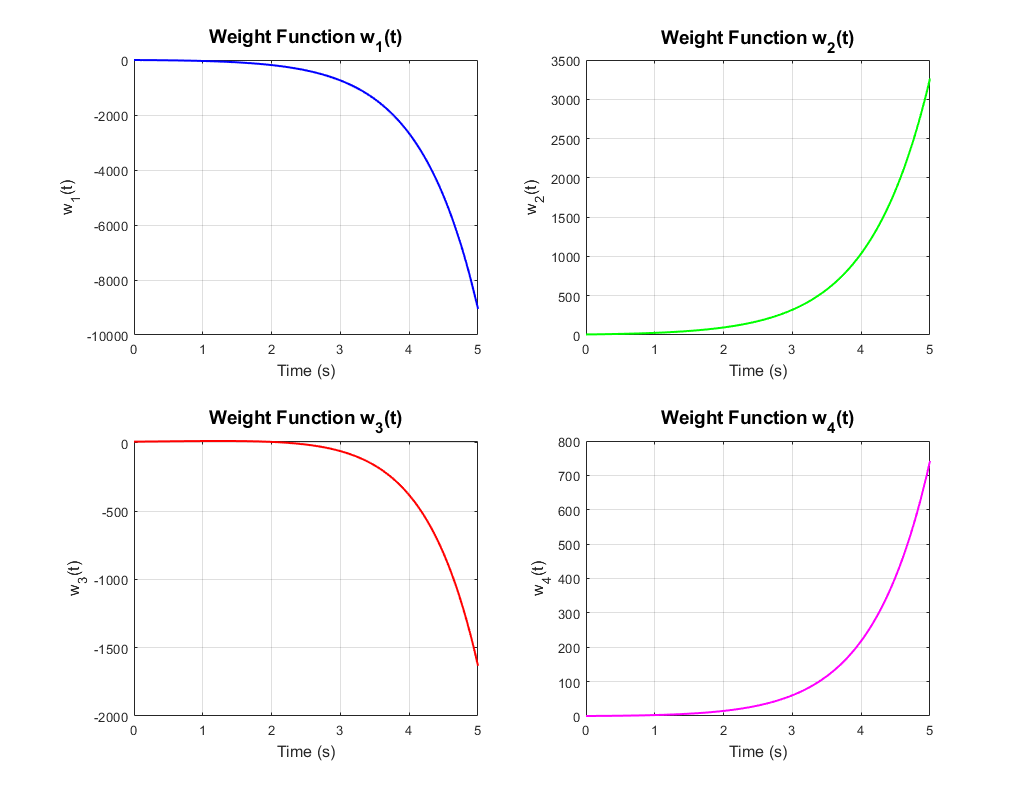
\includegraphics[scale=0.585]{1task_wi.png}
        \captionsetup{skip=0pt}
        \caption{Графики весовых функций $w_k(t)$}
        \label{fig:1task_wi}
    \end{figure}
    \begin{figure}[H]
        \centering
        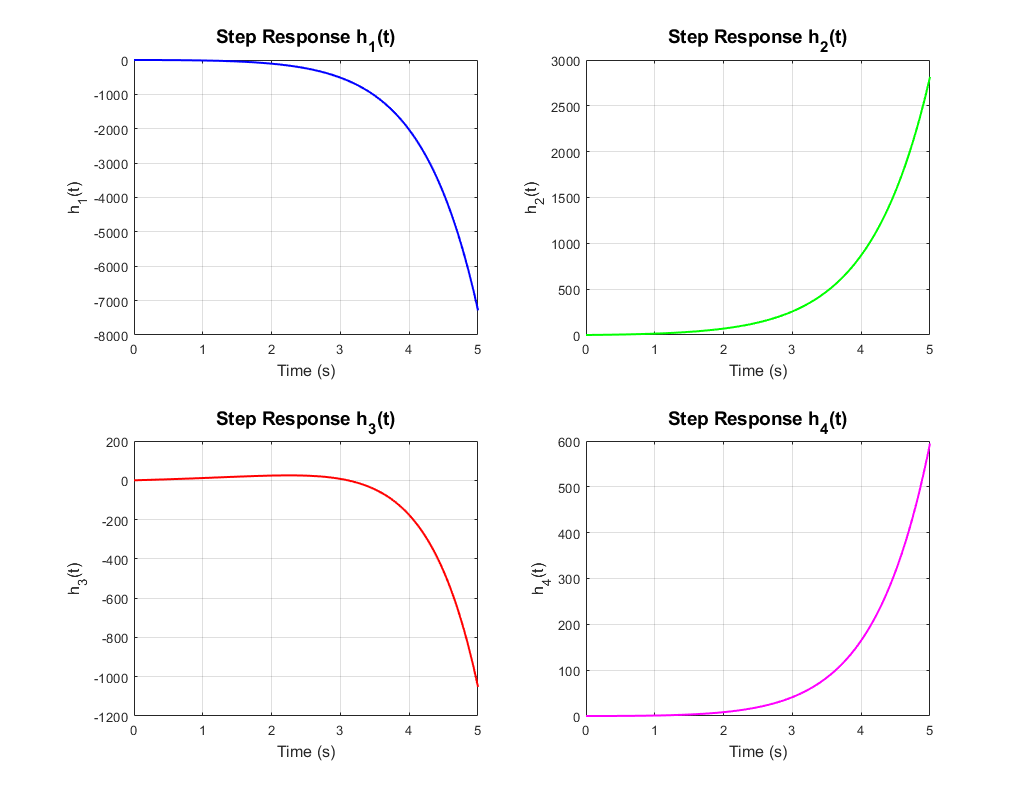
\includegraphics[scale=0.585]{1task_hi.png}
        \captionsetup{skip=0pt}
        \caption{Графики переходных функций $h_k(t)$}
        \label{fig:1task_hi}
    \end{figure}


    \subsection{Частотные характеристики системы}
    Выведем аналитические выражения частотных характеристик системы,
    таких как АЧХ, ФЧХ, ЛАЧХ, ЛФЧХ. АЧХ находим по формуле
    $$
    A_k(\omega)=|W_{l,m}(i\omega)|=\sqrt{\operatorname{Re}^2\left\{ W_{l,m}(i\omega)\right\}+\operatorname{Im}^2\left\{ W_{l,m}(i\omega) \right\}}
    $$
    Найдем $A_1(\omega)$
    $$
    A_1\left( \omega \right)=|W_{1,1}(i\omega)|=\bigg|\dfrac{-i\omega-11}{(i\omega-1)^2}\bigg|,
    $$
    Приведем $W_{1,1}(i\omega)$ к виду суммы реальной и мнимой частей. Домножим числитель и знаменатель
    на комплексно сопряженное к знаменателю число. Упростим выражение и выразим действительную и мнимую части.
    В конце вычислим $A_1(\omega)$
    $$
    W_{1,1}(i\omega)=\dfrac{\left(-i\omega-11\right)\left( i\omega+1 \right)^2}{(i\omega-1)^2\left( i\omega+1 \right)^2}=\dfrac{13\omega^2-11+\left( \omega^3-23\omega \right)i}{\omega^4+2\omega^2+1}=
    \dfrac{13\omega^2-11}{\left( \omega^2+1 \right)^2}+\dfrac{\omega^3-23\omega}{\left(\omega^2+1\right)^2}i,
    $$
    $$
    A_1(\omega)=\sqrt{\left( \dfrac{13\omega^2-11}{\left( \omega^2+1 \right)^2} \right)^2+\left( \dfrac{\omega^3-23\omega}{\left( \omega^2+1 \right)^2} \right)^2}=\dfrac{\sqrt{\omega^6+123\omega^4+243\omega^2+121}}{\left( \omega^2+1 \right)^2};
    $$
    Вычислим оставшиеся $A_k\left( \omega \right)$ аналогично. Сначала приведем $W_{l,m}(i\omega)$ к нужному виду
    \begin{align*}
    &W_{1,2}(i\omega)=\dfrac{\left(7i\omega-4\right)\left( i\omega+1 \right)^2}{(i\omega-1)^2\left( i\omega+1 \right)^2}=\dfrac{18\omega^2-4}{\left( \omega^2+1 \right)^2}+\dfrac{-7\omega^3+15\omega}{\left( \omega^2+1 \right)^2}i,\\
    &W_{2,1}(i\omega)=\dfrac{\left(9i\omega-13\right)\left( i\omega+1 \right)^2}{\left( i\omega-1 \right)^2\left( i\omega+1 \right)^2}=\dfrac{31\omega^2-13}{\left( \omega^2+1 \right)^2}+\dfrac{-9\omega^3+35\omega}{\left( \omega^2+1 \right)^2}i,\\
    &W_{2,2}(i\omega)=\dfrac{\left( i\omega+1 \right)^2}{\left( i\omega-1 \right)^2\left( i\omega+1 \right)^2}=\dfrac{-\omega^2+1}{\left( \omega^2+1 \right)^2}+\dfrac{2\omega}{\left( \omega^2+1 \right)^2}i;
    \end{align*}
    Запишем оставшиеся $A_k(\omega)$
    \begin{align*}
        &A_2\left( \omega \right)=|W_{1,2}(i\omega)|=\bigg|\dfrac{18\omega^2-4}{\left( \omega^2+1 \right)^2}+\dfrac{-7\omega^3+15\omega}{\left( \omega^2+1 \right)^2}i\bigg|,\\
        &A_3(\omega)=|W_{2,1}(i\omega)|=\bigg|\dfrac{31\omega^2-13}{\left( \omega^2+1 \right)^2}+\dfrac{-9\omega^3+35\omega}{\left( \omega^2+1 \right)^2}i\bigg|,\\
        &A_4\left( \omega \right)=|W_{2,2}(i\omega)|=\bigg|\dfrac{-\omega^2+1}{\left( \omega^2+1 \right)^2}+\dfrac{2\omega}{\left( \omega^2+1 \right)^2}i\bigg|;
    \end{align*}
    Вычислим АЧХ
    \begin{align*}
    &A_2\left( \omega \right)=\dfrac{\sqrt{\left( 18\omega^2-4 \right)^2+\left( -7\omega^3+15\omega \right)^2}}{\left( \omega^2+1 \right)^2}=\dfrac{\sqrt{49\omega^6+114\omega^4+81\omega^2+16}}{\left( \omega^2+1 \right)^2},\\
    &A_3(\omega)=\dfrac{\sqrt{\left( 31\omega^2-13 \right)^2+\left( -9\omega^3+35\omega \right)^2}}{\left( \omega^2+1 \right)^2}=\dfrac{\sqrt{81\omega^6+331\omega^4+419\omega^2+169}}{\left( \omega^2+1 \right)^2},\\
    &A_4\left( \omega \right)=\dfrac{\sqrt{\left( -\omega^2+1 \right)^2+\left( 2\omega \right)^2}}{\left( \omega^2+1 \right)^2}=\dfrac{\omega^2+1}{\left( \omega^2+1 \right)^2}=\dfrac{1}{\omega^2+1};
    \end{align*}
    ЛАЧХ ищется по формуле
    $$
    L_k(\omega)=20\log_{10}\left( A_k(\omega) \right)
    $$
    Запишем все $L_k(\omega)$
    \begin{align*}
        &L_1(\omega)=20\log_{10}\left( A_1(\omega) \right)=20\log_{10}\left( \dfrac{\sqrt{\omega^6+123\omega^4+243\omega^2+121}}{\left( \omega^2+1 \right)^2} \right),\\
        &L_2(\omega)=20\log_{10}\left( A_2(\omega) \right)=20\log_{10}\left( \dfrac{\sqrt{49\omega^6+114\omega^4+81\omega^2+16}}{\left( \omega^2+1 \right)^2} \right),\\
        &L_3\left( \omega \right)=20\log_{10}\left( A_3(\omega) \right)=20\log_{10}\left( \dfrac{\sqrt{81\omega^6+331\omega^4+419\omega^2+169}}{\left( \omega^2+1 \right)^2} \right),\\
        &L_4(\omega)=20\log_{10}\left( A_4(\omega) \right)=20\log_{10}\left( \dfrac{1}{\omega^2+1} \right);
    \end{align*}
    Таким образом, пользуясь свойствами логарифмов
    \begin{align*}
    &L_1(\omega)=10\log_{10}\left( \omega^6+123\omega^4+243\omega^2+121 \right)-40\log_{10}\left( \omega^2+1 \right),\\
    &L_2\left( \omega \right)=10\log_{10}\left( 49\omega^6+114\omega^4+81\omega^2+16 \right)-40\log_{10}\left( \omega^2+1 \right),\\
    &L_3\left( \omega \right)=10\log_{10}\left( 81\omega^6+331\omega^4+419\omega^2+169 \right)-40\log_{10}\left( \omega^2+1 \right),\\
    &L_4\left( \omega \right)=-20\log_{10}\left( \omega^2+1 \right);
    \end{align*}
    ФЧХ ищется по формуле
    $$
    \varphi_k(\omega)=\arctan\left(\dfrac{\operatorname{Im}\left\{ W_{l,m}(i\omega) \right\}}{\operatorname{Re}\left\{ W_{l,m}(i\omega)\right\}}\right)
    $$
    У всех $W_{l,m}(i\omega)$ одинаковые знаментали у действительных и мнимых частей. При делении
    мнимой части на действительную знаменатели будут сокращаться. Останутся только отношения числителей.
    Таким образом, запишем $\varphi_k$
    \begin{align*}
        &\varphi_1(\omega)=\arctan\left(\dfrac{\operatorname{Im}_\text{ч}\left\{ W_{1,1}(i\omega) \right\}}{\operatorname{Re}_\text{ч}\left\{ W_{1,1}(i\omega)\right\}}\right)=
        \arctan\left( \dfrac{\omega^3-23\omega}{13\omega^2-11} \right),\\
        &\varphi_1(\omega)=\arctan\left(\dfrac{\operatorname{Im}_\text{ч}\left\{ W_{1,2}(i\omega) \right\}}{\operatorname{Re}_\text{ч}\left\{ W_{1,2}(i\omega)\right\}}\right)=
        \arctan\left( \dfrac{-7\omega^3+15\omega}{18\omega^2-4} \right),\\
        &\varphi_1(\omega)=\arctan\left(\dfrac{\operatorname{Im}_\text{ч}\left\{ W_{2,1}(i\omega) \right\}}{\operatorname{Re}_\text{ч}\left\{ W_{2,1}(i\omega)\right\}}\right)=
        \arctan\left( \dfrac{-9\omega^3+35\omega}{31\omega^2-13} \right),\\
        &\varphi_1(\omega)=\arctan\left(\dfrac{\operatorname{Im}_\text{ч}\left\{ W_{2,2}(i\omega) \right\}}{\operatorname{Re}_\text{ч}\left\{ W_{2,2}(i\omega)\right\}}\right)=
        \arctan\left( \dfrac{2\omega}{-\omega^2+1} \right);
    \end{align*}
    ЛФЧХ имеют такие же аналитические выражения, как и ФЧХ, только вместо частот $\omega$ используется логарифмическая шкала $\log_{10}\left( \omega \right)$.


    \subsection{Графическое представление частотных характеристик}
    Построим графики по расчитанным ранее характеристикам
    \begin{figure}[H]
        \centering
        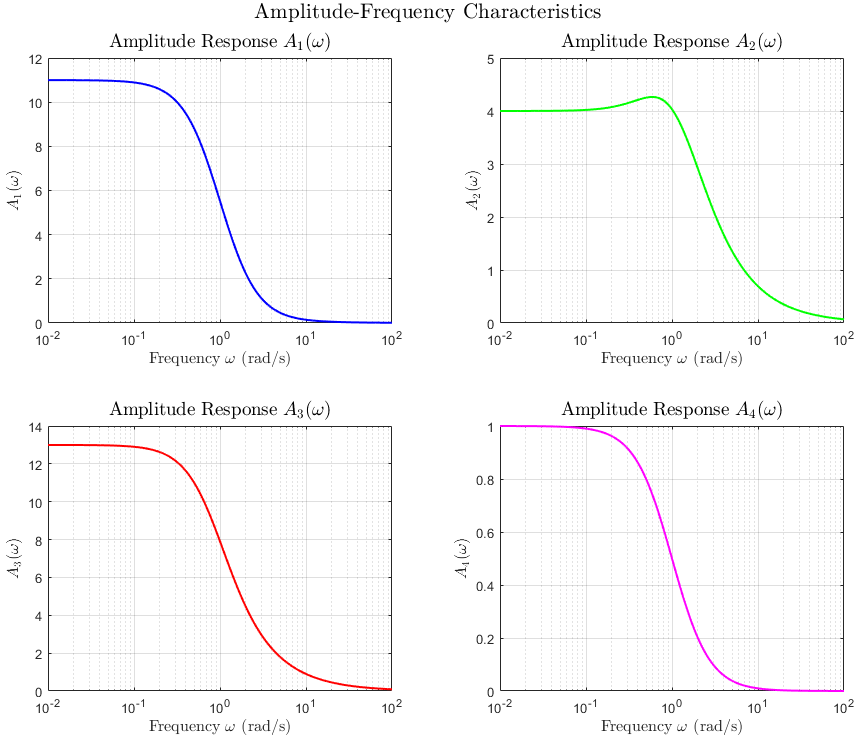
\includegraphics[scale=0.585]{1task_afr.png}
        \captionsetup{skip=0pt}
        \caption{Графики АЧХ $A_k(\omega)$}
        \label{fig:1task_afr}
    \end{figure}
    \begin{figure}[H]
        \centering
        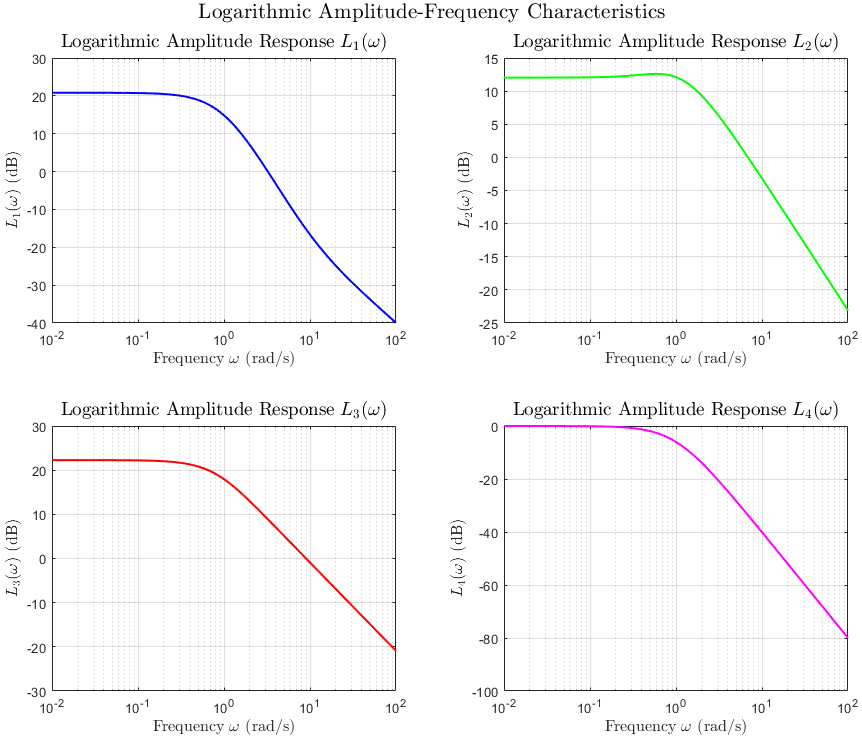
\includegraphics[scale=0.585]{1task_lafr.png}
        \captionsetup{skip=0pt}
        \caption{Графики ЛАЧХ $L_k(\omega)$}
        \label{fig:1task_lafr}
    \end{figure}
    \begin{figure}[H]
        \centering
        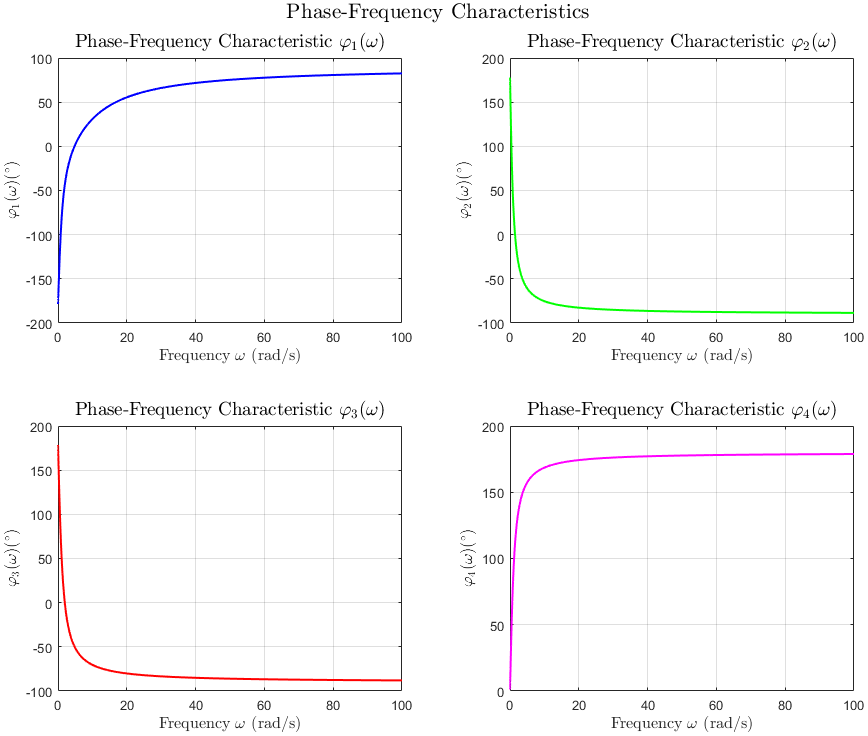
\includegraphics[scale=0.585]{1task_phii.png}
        \captionsetup{skip=0pt}
        \caption{Графики ФЧХ $\varphi_k(t)$}
        \label{fig:1task_phii}
    \end{figure}
    \begin{figure}[H]
        \centering
        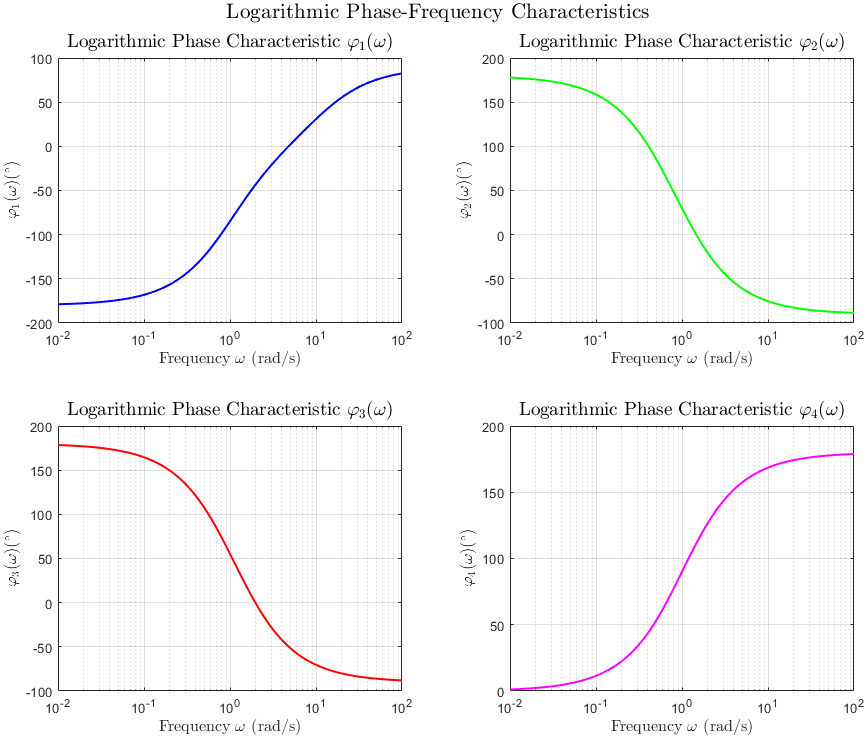
\includegraphics[scale=0.585]{1task_lphii.png}
        \captionsetup{skip=0pt}
        \caption{Графики ЛФЧХ $\varphi_k(t),x=\log_{10}\left( \omega \right)$}
        \label{fig:1task_lphii}
    \end{figure}
    \noindent Результаты похожи на апериодические звенья 2-го порядка.


    \section{Задание 2. Синтез следящего управления в условиях внешних возмущений для многоканальной системы}
    Рассмотрим многоканальную систему
    $$
    \begin{cases}
        \dot{x}=Ax+Bu+B_ff_1,\\
        z=C_zx+D_zu-g,\\
        y=Cx+Du+D_ff_2,
    \end{cases} x(0)=\begin{bmatrix}
        1\\1
    \end{bmatrix}
    $$
    при
    $$
    A=\begin{bmatrix}
        0 &1\\
        -1 &2
    \end{bmatrix},\ B=\begin{bmatrix}
        1 &2\\
        -3 &3
    \end{bmatrix},\ C=\begin{bmatrix}
        2 &1\\
        3 &-2
    \end{bmatrix},\ D=\begin{bmatrix}
        -2 &0\\
        0 &1
    \end{bmatrix},
    $$
    $$
    B_f=\begin{bmatrix}
        1 &2\\
        -1 &3
    \end{bmatrix},\ D_f=\begin{bmatrix}
        1 &0\\
        0 &-1
    \end{bmatrix},\ C_z=\begin{bmatrix}
        4 &2\\
        -1 &1
    \end{bmatrix},\ D_z=\begin{bmatrix}
        2 &0\\
        0 &1
    \end{bmatrix},
    $$
    $$
    f_1(t)=\begin{bmatrix}
        9\sin\left( 3t \right)\\
        3\cos\left( 2t \right)
    \end{bmatrix},\ f_2(t)=\begin{bmatrix}
        6\cos\left( 2t \right)\\
        8\sin\left( 3t \right)
    \end{bmatrix},\ g(t)=\begin{bmatrix}
        3\cos\left( 4t \right)\\
        6\sin\left( 4t \right)
    \end{bmatrix};
    $$
    К измерению доступны только величины $y(t),g(t)$. Программа находится в приложении Б на листинге \ref{task2}.


    \subsection{Структурные свойства многоканальной системы}
    ...


    \section{Общий вывод по работе}
    ...


    \section{Приложение А}
    \begin{lstlisting}[label=task1, caption={Программа для задания 1}]
    % plant parameters
    A=[0 1; -1 2];
    B=[1 2; -3 3];
    C=[2 1; 3 -2];
    D=[0 0; 0 0];

    % A eig
    A_eig = eig(A)

    % W(s)
    sys = ss(A, B, C, D);
    W_s = tf(sys)

    % zeros
    zeros = zero(sys)

    % poles
    poles = pole(sys)

    % Jordan matrix
    [P, J] = jordan(A)
    B_J = inv(P) * B
    C_J = C * P

    % out
    U = [B A*B];
    U_out = [C*U D]
    rank(U_out)

    % time
    t = 0:0.01:5;

    % w(t)
    w1 = -exp(t) - 12*t.*exp(t);
    w2 = 7*exp(t) + 3*t.*exp(t);
    w3 = 9*exp(t) - 4*t.*exp(t);
    w4 = t.*exp(t);

    % h(t)
    h1 = -12*t.*exp(t) + 11*exp(t) - 11;
    h2 = 3*t.*exp(t) + 4*exp(t) - 4;
    h3 = -4*t.*exp(t) + 13*exp(t) - 13;
    h4 = t.*exp(t) - exp(t) + 1;

    % w(t) renders
    figure;
    subplot(2,2,1)
    plot(t, w1, 'b', 'LineWidth', 1.5); grid on;
    xlabel('Time (s)', 'Interpreter','latex', 'FontSize', 12);
    ylabel('$w_1(t)$', 'Interpreter','latex', 'FontSize', 12);
    title('Weight Function $w_1(t)$', 'Interpreter','latex', 'FontSize', 14);

    subplot(2,2,2)
    plot(t, w2, 'g', 'LineWidth', 1.5); grid on;
    xlabel('Time (s)', 'Interpreter','latex', 'FontSize', 12);
    ylabel('$w_2(t)$', 'Interpreter','latex', 'FontSize', 12);
    title('Weight Function $w_2(t)$', 'Interpreter','latex', 'FontSize', 14);

    subplot(2,2,3)
    plot(t, w3, 'r', 'LineWidth', 1.5); grid on;
    xlabel('Time (s)', 'Interpreter','latex', 'FontSize', 12);
    ylabel('$w_3(t)$', 'Interpreter','latex', 'FontSize', 12);
    title('Weight Function $w_3(t)$', 'Interpreter','latex', 'FontSize', 14);

    subplot(2,2,4)
    plot(t, w4, 'm', 'LineWidth', 1.5); grid on;
    xlabel('Time (s)', 'Interpreter','latex', 'FontSize', 12);
    ylabel('$w_4(t)$', 'Interpreter','latex', 'FontSize', 12);
    title('Weight Function $w_4(t)$', 'Interpreter','latex', 'FontSize', 14);

    % h(t) renders
    figure;
    subplot(2,2,1)
    plot(t, h1, 'b', 'LineWidth', 1.5); grid on;
    xlabel('Time (s)', 'Interpreter','latex', 'FontSize', 12);
    ylabel('$h_1(t)$', 'Interpreter','latex', 'FontSize', 12);
    title('Step Response $h_1(t)$', 'Interpreter','latex', 'FontSize', 14);

    subplot(2,2,2)
    plot(t, h2, 'g', 'LineWidth', 1.5); grid on;
    xlabel('Time (s)', 'Interpreter','latex', 'FontSize', 12);
    ylabel('$h_2(t)$', 'Interpreter','latex', 'FontSize', 12);
    title('Step Response $h_2(t)$', 'Interpreter','latex', 'FontSize', 14);

    subplot(2,2,3)
    plot(t, h3, 'r', 'LineWidth', 1.5); grid on;
    xlabel('Time (s)', 'Interpreter','latex', 'FontSize', 12);
    ylabel('$h_3(t)$', 'Interpreter','latex', 'FontSize', 12);
    title('Step Response $h_3(t)$', 'Interpreter','latex', 'FontSize', 14);

    subplot(2,2,4)
    plot(t, h4, 'm', 'LineWidth', 1.5); grid on;
    xlabel('Time (s)', 'Interpreter','latex', 'FontSize', 12);
    ylabel('$h_4(t)$', 'Interpreter','latex', 'FontSize', 12);
    title('Step Response $h_4(t)$', 'Interpreter','latex', 'FontSize', 14);

    % freq
    omega = logspace(-2, 2, 1000);

    % A(w)
    A1 = sqrt(omega.^6 + 123*omega.^4 + 243*omega.^2 + 121) ./ (omega.^2 + 1).^2;
    A2 = sqrt(49*omega.^6 + 114*omega.^4 + 81*omega.^2 + 16) ./ (omega.^2 + 1).^2;
    A3 = sqrt(81*omega.^6 + 331*omega.^4 + 419*omega.^2 + 169) ./ (omega.^2 + 1).^2;
    A4 = 1 ./ (omega.^2 + 1);

    % A(w) renders
    figure;

    subplot(2,2,1)
    semilogx(omega, A1, 'b', 'LineWidth', 1.5); grid on;
    xlabel('Frequency $\omega$ (rad/s)', 'Interpreter','latex', 'FontSize', 12);
    ylabel('$A_1(\omega)$', 'Interpreter','latex', 'FontSize', 12);
    title('Amplitude Response $A_1(\omega)$', 'Interpreter','latex', 'FontSize', 14);

    subplot(2,2,2)
    semilogx(omega, A2, 'g', 'LineWidth', 1.5); grid on;
    xlabel('Frequency $\omega$ (rad/s)', 'Interpreter','latex', 'FontSize', 12);
    ylabel('$A_2(\omega)$', 'Interpreter','latex', 'FontSize', 12);
    title('Amplitude Response $A_2(\omega)$', 'Interpreter','latex', 'FontSize', 14);

    subplot(2,2,3)
    semilogx(omega, A3, 'r', 'LineWidth', 1.5); grid on;
    xlabel('Frequency $\omega$ (rad/s)', 'Interpreter','latex', 'FontSize', 12);
    ylabel('$A_3(\omega)$', 'Interpreter','latex', 'FontSize', 12);
    title('Amplitude Response $A_3(\omega)$', 'Interpreter','latex', 'FontSize', 14);

    subplot(2,2,4)
    semilogx(omega, A4, 'm', 'LineWidth', 1.5); grid on;
    xlabel('Frequency $\omega$ (rad/s)', 'Interpreter','latex', 'FontSize', 12);
    ylabel('$A_4(\omega)$', 'Interpreter','latex', 'FontSize', 12);
    title('Amplitude Response $A_4(\omega)$', 'Interpreter','latex', 'FontSize', 14);

    sgtitle('Amplitude-Frequency Characteristics', 'Interpreter','latex', 'FontSize', 16);

    % L(w)
    L1 = 10 * log10(omega.^6 + 123*omega.^4 + 243*omega.^2 + 121) - 40 * log10(omega.^2 + 1);
    L2 = 10 * log10(49*omega.^6 + 114*omega.^4 + 81*omega.^2 + 16) - 40 * log10(omega.^2 + 1);
    L3 = 10 * log10(81*omega.^6 + 331*omega.^4 + 419*omega.^2 + 169) - 40 * log10(omega.^2 + 1);
    L4 = -20 * log10(omega.^2 + 1);

    % L(w) renders
    figure;

    subplot(2,2,1)
    semilogx(omega, L1, 'b', 'LineWidth', 1.5); grid on;
    xlabel('Frequency $\omega$ (rad/s)', 'Interpreter','latex', 'FontSize', 12);
    ylabel('$L_1(\omega)$ (dB)', 'Interpreter','latex', 'FontSize', 12);
    title('Logarithmic Amplitude Response $L_1(\omega)$', 'Interpreter','latex', 'FontSize', 14);

    subplot(2,2,2)
    semilogx(omega, L2, 'g', 'LineWidth', 1.5); grid on;
    xlabel('Frequency $\omega$ (rad/s)', 'Interpreter','latex', 'FontSize', 12);
    ylabel('$L_2(\omega)$ (dB)', 'Interpreter','latex', 'FontSize', 12);
    title('Logarithmic Amplitude Response $L_2(\omega)$', 'Interpreter','latex', 'FontSize', 14);

    subplot(2,2,3)
    semilogx(omega, L3, 'r', 'LineWidth', 1.5); grid on;
    xlabel('Frequency $\omega$ (rad/s)', 'Interpreter','latex', 'FontSize', 12);
    ylabel('$L_3(\omega)$ (dB)', 'Interpreter','latex', 'FontSize', 12);
    title('Logarithmic Amplitude Response $L_3(\omega)$', 'Interpreter','latex', 'FontSize', 14);

    subplot(2,2,4)
    semilogx(omega, L4, 'm', 'LineWidth', 1.5); grid on;
    xlabel('Frequency $\omega$ (rad/s)', 'Interpreter','latex', 'FontSize', 12);
    ylabel('$L_4(\omega)$ (dB)', 'Interpreter','latex', 'FontSize', 12);
    title('Logarithmic Amplitude Response $L_4(\omega)$', 'Interpreter','latex', 'FontSize', 14);

    sgtitle('Logarithmic Amplitude-Frequency Characteristics', 'Interpreter','latex', 'FontSize', 16);

    % phi(w)
    phi1 = atan2(omega.^3 - 23*omega, 13*omega.^2 - 11);
    phi2 = atan2(-7*omega.^3 + 15*omega, 18*omega.^2 - 4);
    phi3 = atan2(-9*omega.^3 + 35*omega, 31*omega.^2 - 13);
    phi4 = atan2(2*omega, -omega.^2 + 1);

    % rad to deg
    phi1 = rad2deg(phi1);
    phi2 = rad2deg(phi2);
    phi3 = rad2deg(phi3);
    phi4 = rad2deg(phi4);

    % phi(w)
    figure;

    subplot(2,2,1)
    plot(omega, phi1, 'b', 'LineWidth', 1.5); grid on;
    xlabel('Frequency $\omega$ (rad/s)', 'Interpreter','latex', 'FontSize', 12);
    ylabel('$\varphi_1(\omega) (^\circ)$', 'Interpreter','latex', 'FontSize', 12);
    title('Phase-Frequency Characteristic $\varphi_1(\omega)$', 'Interpreter','latex', 'FontSize', 14);

    subplot(2,2,2)
    plot(omega, phi2, 'g', 'LineWidth', 1.5); grid on;
    xlabel('Frequency $\omega$ (rad/s)', 'Interpreter','latex', 'FontSize', 12);
    ylabel('$\varphi_2(\omega) (^\circ)$', 'Interpreter','latex', 'FontSize', 12);
    title('Phase-Frequency Characteristic $\varphi_2(\omega)$', 'Interpreter','latex', 'FontSize', 14);

    subplot(2,2,3)
    plot(omega, phi3, 'r', 'LineWidth', 1.5); grid on;
    xlabel('Frequency $\omega$ (rad/s)', 'Interpreter','latex', 'FontSize', 12);
    ylabel('$\varphi_3(\omega) (^\circ)$', 'Interpreter','latex', 'FontSize', 12);
    title('Phase-Frequency Characteristic $\varphi_3(\omega)$', 'Interpreter','latex', 'FontSize', 14);

    subplot(2,2,4)
    plot(omega, phi4, 'm', 'LineWidth', 1.5); grid on;
    xlabel('Frequency $\omega$ (rad/s)', 'Interpreter','latex', 'FontSize', 12);
    ylabel('$\varphi_4(\omega) (^\circ)$', 'Interpreter','latex', 'FontSize', 12);
    title('Phase-Frequency Characteristic $\varphi_4(\omega)$', 'Interpreter','latex', 'FontSize', 14);

    sgtitle('Phase-Frequency Characteristics', 'Interpreter','latex', 'FontSize', 16);

    % log phi(w)
    figure;

    subplot(2,2,1)
    semilogx(omega, phi1, 'b', 'LineWidth', 1.5); grid on;
    xlabel('Frequency $\omega$ (rad/s)', 'Interpreter','latex', 'FontSize', 12);
    ylabel('$\varphi_1(\omega) (^\circ)$', 'Interpreter','latex', 'FontSize', 12);
    title('Logarithmic Phase Characteristic $\varphi_1(\omega)$', 'Interpreter','latex', 'FontSize', 14);

    subplot(2,2,2)
    semilogx(omega, phi2, 'g', 'LineWidth', 1.5); grid on;
    xlabel('Frequency $\omega$ (rad/s)', 'Interpreter','latex', 'FontSize', 12);
    ylabel('$\varphi_2(\omega) (^\circ)$', 'Interpreter','latex', 'FontSize', 12);
    title('Logarithmic Phase Characteristic $\varphi_2(\omega)$', 'Interpreter','latex', 'FontSize', 14);

    subplot(2,2,3)
    semilogx(omega, phi3, 'r', 'LineWidth', 1.5); grid on;
    xlabel('Frequency $\omega$ (rad/s)', 'Interpreter','latex', 'FontSize', 12);
    ylabel('$\varphi_3(\omega) (^\circ)$', 'Interpreter','latex', 'FontSize', 12);
    title('Logarithmic Phase Characteristic $\varphi_3(\omega)$', 'Interpreter','latex', 'FontSize', 14);

    subplot(2,2,4)
    semilogx(omega, phi4, 'm', 'LineWidth', 1.5); grid on;
    xlabel('Frequency $\omega$ (rad/s)', 'Interpreter','latex', 'FontSize', 12);
    ylabel('$\varphi_4(\omega) (^\circ)$', 'Interpreter','latex', 'FontSize', 12);
    title('Logarithmic Phase Characteristic $\varphi_4(\omega)$', 'Interpreter','latex', 'FontSize', 14);

    sgtitle('Logarithmic Phase-Frequency Characteristics', 'Interpreter','latex', 'FontSize', 16);
    \end{lstlisting}


    \section{Приложение Б}
    \begin{lstlisting}[label=task2, caption={Программа для задания 2}]
        tbd
    \end{lstlisting}
\end{document}